%!TEX root = main.tex
\begin{figure*}[t]
\centering
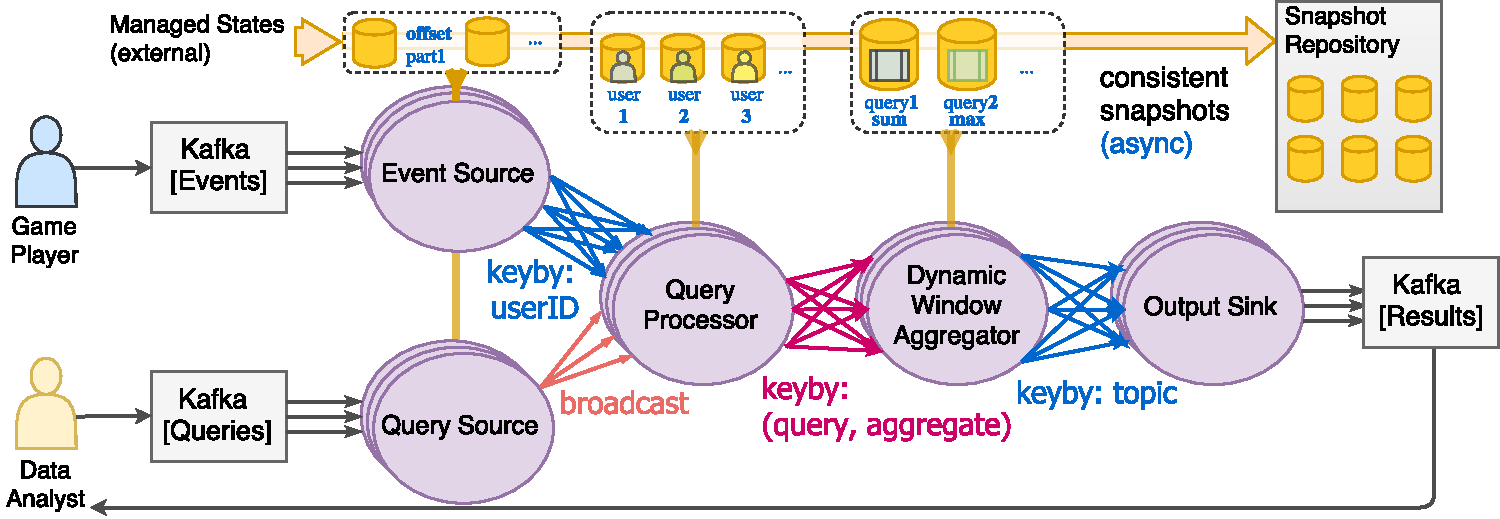
\includegraphics[width=\textwidth]{figures/rbea.pdf}
\caption{A Flink pipeline implementing an adhoc standing query execution service at King} 
\label{fig:rbea}
\vspace{-4mm}
\end{figure*}

\begin{figure}
\centering
\subcaptionbox{Snapshot Duration vs Total Size \stefan{I think the information on how many nodes this was running should be part of the plot or the footer. This is important to interpret the performance and makes the plot more self-contained}}{%
  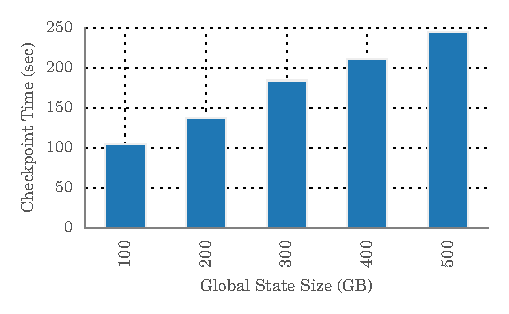
\includegraphics[width=0.45\textwidth]{figures/cp1checkpoint.pdf}%
  }\par\medskip
\subcaptionbox{Total Alignment Time vs Snapshot Size}{%
  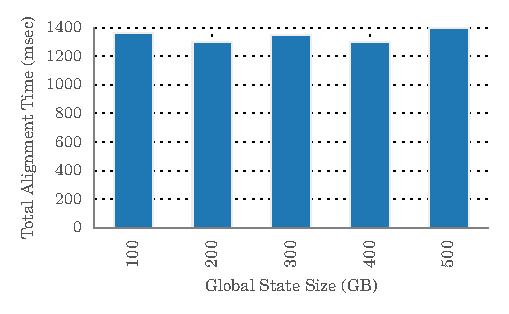
\includegraphics[width=0.45\textwidth]{figures/cp1align.pdf}%
  }\par\medskip
\subcaptionbox{Total Alignment Time (Detailed) vs Parallelism}{%
  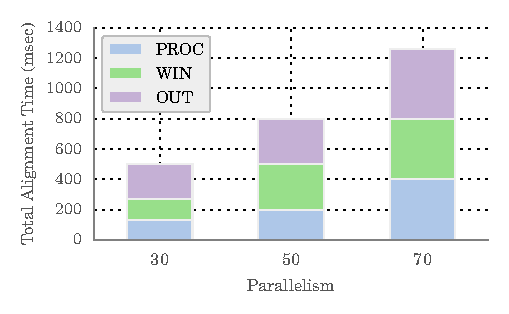
\includegraphics[width=0.45\textwidth]{figures/cp2align.pdf}%
  }
\caption{RBEA Deployment Measurements on Snapshots }
\label{fig:kingmetrics}
\end{figure}


\section{Large-Scale Deployments}
\label{sec:evaluation}


Flink is currently one of the most widespread systems in production\gyula{is this claim true?}, serving as a the core engine for continuous data processing. Large-scale deployments range from dozens to 1000s of nodes and serve a wide variety of data management and analysis needs. In this section, we present a few examples of how Flink's lightweight state management features are being used in practice, within large deployments and also present live metrics and insights.

\paris{@Kostas feel free to edit this section. No need to add your tag. I can see the diffs in sharelatex and fix afterwards}

\para{Alibaba} is actively using Flink in their production cluster (1000+ nodes) to support their critical search service \cite{CUSTOM:web/alibaba} and keep search results and recommendation as fresh and relevant to their active retail catalogue as possible.

%King.com

%\para{Zalando}

%\para{Uber}


%\para{Bouygues Telecom}

%\para{ResearchGate}

%Uber, Netflix, ING, MediaMath, New Relic



\subsection{A Real-Time Analytics Platform}

The Rule-Based Event Aggregator (RBEA) by King (MidasPlayer AB) \cite{CUSTOM:web/kingrbea}, is a reliable live service that is implemented on Apache Flink and used daily by data analysts and database engineers for more than a year. RBEA showcases how Flink's stateful processing capabilities can be exploited to build a highly dynamic live service that allows analysts to declare and run standing queries on large-scale mobile event streams, backed by Flink's consistent state. In essence, the service covers several fundamental needs of data analysts: 1) instant access to timely user data, 2) the ability to deploy declarative standing queries, 3) creation and manipulation of custom aggregation metrics, 4) a transparent execution, eliminating the need for technical expertise.

\subsubsection{The RBEA Service Pipeline}
\autoref{fig:rbea} depicts an overview of the end-to-end Flink pipeline that implements the core of the service. There are two types of streams, ingested from Kafka: a) an \texttt{Event} stream originating from  user actions (circa 30 billion events per day) such as \texttt{GameStarted} or \texttt{GameEnded} and b) a \texttt{Query} stream containing standing queries in the form of serialized scripts written by data analysts through the frontend of RBEA in a provided DSL (e.g., using Groovy or Java). Standing queries in RBEA allow analysts to access user-specific data and event sequences as well as triggering special aggregation logic on sliding data windows (respecting the semantics of Flink's implementation of the Dataflow Model \cite{akidau2015dataflow}). 

Standing queries are forwarded and executed inside \texttt{[Query Processor]} instances which hold managed state entries per user accumulated by any stateful processing logic. A ``broadcast'' data dependency is being used to submit each query to all instances of the \texttt{[Query Processor]} so it can be executed in parallel while game events are otherwise partitioned by their associated user ids to the same operator. Aggregation calls in RBEA's standing query DSL trigger output events from \texttt{[Query Processor]} operator which are subsequently consumed by the \texttt{[Dynamic Window Aggregator]}. This operator assigns the aggregator events to the current event-time window and also applies the actual aggregation logic. Aggregated values are sent to the \texttt{[Output sink]} operator which writes them directly to an external database or Kafka. 

%failures during script execution need to be backpropagated to all the parallel instances in order the remove all instances of the broken scripts. Iterations are used to implement the failure propagation logic.


\subsubsection{Performance Metrics and Insights} We gathered several performance metrics from live deployments of RBEA over weeks of its runtime in order to present insights and discuss the performance costs related to snapshotting, as well as the factors that can affect those costs. All deployments of RBEA are currently using Flink (v.1.2.0) and Task Managers were configured to use the out-of-core backend (on RocksDB) which also enables asynchronous snapshotting. The performance of Flink's state management layer, that we discuss bellow,  have been evaluated to address two main questions: 1) What affects  snapshotting latency?, and 2) How and when is normal execution impacted?

\para{What affects snapshotting latency?} \\
We extracted measurements from five different RBEA deployments with fixed parallelism $\pi = 70$ ranging from 100 to 500 GB global state respectively (addressing different mobile applications). \autoref{fig:kingmetrics}(a) depicts the overall time it takes to undertake a full snapshot asynchronously for each different version. Mind that this simply measures the time difference between the invocation of a snapshot (epoch marker injection) and the moment all operators notify back they have completed it through the asynchronous backend calls. Since snapshots are asynchronously committed these latencies are not translated into execution impact costs. Alignment is the sole-most factor of the snapshotting process that can impact normal execution. \autoref{fig:kingmetrics}(b) summarizes the overall time RBEA task instances have spent in \emph{alignment} mode, inducing an overall average delay of 1.3 seconds. Furthermore, another conclusion we can make from the same metrics is that the global state size does not affect alignment times and as a result the normal execution of a pipeline, given that state is asynchronously snapshotted.

\para{How and when is normal execution impacted?} \\
Alignment enforces partial blocking  on input channels of tasks and thus, more channels can yield a higher runtime latency cost. Evidently, the number of parallel subtasks $\pi$ in a pipeline can potentially affect alignment. \autoref{fig:kingmetrics})(c) shows the total times spent aligning in different RBEA deployments of fixed size (200GB) having varying parallelism. The overall alignment time is clearly proportional to two factors: 1) the number of shuffles encountered along a pipeline (i.e. \texttt{keyby} between the \texttt{PROCESSOR}, \texttt{WINDOW} and \texttt{OUTPUT} operators respectively), each of which introduces its own alignment stage and 2) the parallelism of the tasks. Nevertheless, we can additionally conclude that potential latency spikes of 1 to 3sec (e.g., in the case of 7 stages with parallelism 70) in pipelines of such large scale are hardly considered to be disrupting or breaking SLAs, especially in highly utilized clusters where actual network spikes and CPU load can cause much more potential disruptions in a continuous pipeline execution.